\documentclass[12pt]{article}
\usepackage[english]{babel}
\usepackage{natbib}
\usepackage{url}
\usepackage[utf8x]{inputenc}

\usepackage{parskip}
\usepackage{fancyhdr}
\usepackage{vmargin}
\setmarginsrb{3 cm}{2.5 cm}{3 cm}{2.5 cm}{1 cm}{1.0 cm}{1 cm}{1.5 cm}

\usepackage[linktocpage=all]{hyperref}
\usepackage{color}   %May be necessary if you want to color links
\usepackage{hyperref}
\hypersetup{
    colorlinks=true, %set true if you want colored links
    linktoc=all,     %set to all if you want both sections and subsections linked
    linkcolor=black,  %choose some color if you want links to stand out
}

\usepackage{float}
\usepackage{caption}
\usepackage{subcaption}
\usepackage{parcolumns}

\usepackage{amsmath}
\usepackage{amssymb}
\usepackage{amsthm}

\usepackage{graphicx}
\graphicspath{{images/}}

\usepackage{booktabs}
\usepackage{bm}

\usepackage{pdfpages}
\usepackage{tocloft}

\title{Group Assignment}                                % Title
\author{
    % TODO: PLEASE INSERT YOUR UNI KEYS HERE FOLLOWED BY '\\'
    Charles Hyland 450411920 \\
    Yiran Jing 460244129 \\
    TODO: JAZLYN!!!
}                               % Author
\date{Semester 1, 2019}                                         % Date

\makeatletter
\let\thetitle\@title
\let\theauthor\@author
\let\thedate\@date
\makeatother

\pagestyle{fancy}
\fancyhf{}
%\rhead{\theauthor}
\lhead{Big Data Tuning Assignment}
\cfoot{\thepage}



\begin{document}

%%%%%%%%%%%%%%%%%%%%%%%%%%%%%%%%%%%%%%%%%%%%%%%%%%%%%%%%%%%%%%%%%%%%%%%%%%%%%%%%%%%%%%%%%

\begin{titlepage}
    \centering
    \vspace*{0.5 cm}
    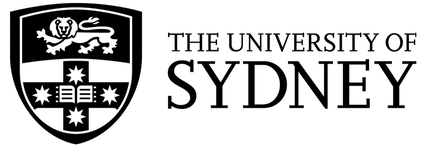
\includegraphics[scale = 0.75]{USYD_LOGO_New.jpg}\\[1.0 cm] % University Logo
    \textsc{\LARGE University of Sydney}\\[2.0 cm]  % University Name
    \textsc{\Large DATA3404}\\[0.5 cm]              % Course Code
    \textsc{\large Data Science Platforms}\\[0.5 cm]                % Course Name
    \rule{\linewidth}{0.2 mm} \\[0.4 cm]
    { \huge \bfseries \thetitle}\\
    \rule{\linewidth}{0.2 mm} \\[1.5 cm]
    
    
        
    \emph{Team members:}\\
    \theauthor
        
    \begin{minipage}{0.45\textwidth}
            
    \end{minipage}\\[2 cm]
    
    {\large \thedate}\\[2 cm]
 
    \vfill
    
\end{titlepage}

%%%%%%%%%%%%%%%%%%%%%%%%%%%%%%%%%%%%%%%%%%%%%%%%%%%%%%%%%%%%%%%%%%%%%%%%%%%%%%%%%%%%%%%%%

\tableofcontents
\pagebreak

%%%%%%%%%%%%%%%%%%%%%%%%%%%%%%%%%%%%%%%%%%%%%%%%%%%%%%%%%%%%%%%%%%%%%%%%%%%%%%%%%%%%%%%%%

\phantomsection
\addcontentsline{toc}{section}{Job Design Documentation}
\section*{Job Design Documentation}
\addcontentsline{toc}{subsection}{Task 1: Top-3 Cessna Models}
\subsection*{Task 1: Top 3 Cessna Models}
\textit{Aircrafts}: A set of tuples with three fields(tail number, manufacturer, and model)\\
\textit{Flights}: : A set of tuples with one field (tail number)

\textbf{\textit{Before:}} 
\begin{enumerate}
  \item Join two data files using \textbf{join} function with join key tail number. 
  
  \item Apply \textbf{FilterFunction} to only return aircrafts with the manufacturer equaled to "CESSNA", and then use \textbf{project} function to project the "model" column only. 
  
  \item After that, apply \textbf{flatMap} with \textbf{CountFlightPerModel} object to produces one for each instance, also add "Cseena" to each instance and abstract the first three digits of each instance to fit the final output format.
  
  \item Then, Group data by the different Cessna models using \textbf{groupBy} function, and for each group use \textbf{sum} to count all the instances of the same Cessna model.
  
  \item Rank Cessna models in descending order using \textbf{sortPartition} function. And return the top 3 Cessna model by \textbf{first}.
\end{enumerate}


\textbf{\textit{After:}}
\begin{enumerate}

%%% setParallelism can be used????? 
 \item Apply \textbf{FilterFunction} to only return aircrafts with the manufacturer equaled to "CESSNA", and then use \textbf{project} function to project the tail number and model columns. 
 
 \item Join two data files using \textbf{join} with \textbf{broadcast hash} the filtered CESSNA model file and then project model column only.  
  
 \item Add \textbf{ReadFields} for the \textbf{CountFlightPerModel} object to specifies the model field is used to compute a result value. After that, apply \textbf{flatMap} with \textbf{CountFlightPerModel} object. And the following steps same as before.
\end{enumerate}









\addcontentsline{toc}{subsection}{Task 2 Average Departure Delay}
\subsection*{Task 2 Average Departure Delay}

\textit{Aircrafts}: A set of tuples with one fields(tail number)\\
\textit{Flights}: : A set of tuples with five field (carrier code, flight date, tail number, scheduled departure, actual departure)\\
\textit{Airlines}: : A set of tuples with three field (carrier code, name, country)\\
A variable named \textit{year} will save the user specific year. (We use 2004 to evaluate). 

\textbf{\textit{Before:}} 
\begin{enumerate}
\item At the beginning, we filter airline dataset by \textbf{FilterFunction} to contain only US Airlines, and then \textbf{project} only two carrier code and name columns(delete "country" column) after this step.
\item Filter the specified year using 'flight date' field of Flights file, and then this field is removed. 
\item Filter out non-delayed flights if actual departure time is not later than scheduled time, and filter out the cancelled flight by catch ParseException within \textbf{FilterFunction}
\item After that, apply \textbf{flatMap} with \textbf{TimeDifferenceMapper} object to
calculate the actual delay time for each delay departure flight. 
\item Join these three dataset to get the the\textit{joinresult} dataset, project only two columns (airline name, length of delay time)

\item Apply \textbf{flatMap} with \textbf{NumMapper} object to produces one for each instance, then, group data by the different US airlines using \textbf{groupBy} function, and for each group use \textbf{sum} to count all the instances of the same US airlines, get the \textit{joinresultNum} dataset

\item Then, Group \textit{joinresult} data by the US airlines using \textbf{groupBy} function, and use \textbf{sum} to get the total length of delay time for each US airline. After that, join this dataset with \textit{joinresultNum} get \textit{joinresultNumSum} dataset. 

\item Group \textit{joinresult} data by the US airlines using \textbf{groupBy} function, and use \textbf{min} to get the min length of delay time for each US airline. After that, join this dataset with \textit{joinresultNumSum} get \textit{joinresultNumSumMin} dataset.

\item Group \textit{joinresult} data by the US airlines using \textbf{groupBy} function, and use \textbf{max} to get the max length of delay time for each US airline. After that, join this dataset with \textit{joinresultNumSumMin} get \textit{joinresultNumSumMinMax} dataset.

\item Apply \textbf{flatMap} with \textbf{AvgMapper} object to get the average delay time for each US airline. Then Rank US airlines in alphabetical order by \textbf{sortPartition} function.

\end{enumerate}

\textbf{\textit{After:}} 

\begin{enumerate}
\item step 1 to 4 same as before, but Rank US airlines in alphabetical order by \textbf{sortPartition} function before join.

\item To join two data files using \textbf{join} with \textbf{broadcast hash} the aircrafts file and the filtered US airlines file, then project only two columns (airline name, length of delay time)

\item After \textbf{groupBy} the US airline result, instand step 6 to 10, we apply \textbf{reduceMap} function with \textbf{Aggregation} function to count the number of delay and the average, min and max delay time for each US airline at the same time. And add \textbf{ForwardedFields} and \textbf{ReadFields} to this object.

\end{enumerate}

\addcontentsline{toc}{subsection}{Task 3: Most Popular Aircraft Types}
\subsection*{Task 3: Most Popular Aircraft Types}
\textit{Aircrafts}: A set of tuples with three fields(tail number, manufacturer, model)\\
\textit{Flights}: : A set of tuples with five field (carrier code, tail number)\\
\textit{Airlines}: : A set of tuples with three field (carrier code, name, country)\\

\textbf{\textit{Before:}} 
\begin{enumerate}
    \item We join the airlines dataset on the flights dataset based on the carrier code. Furthermore, we restrict the output to only include the airline name and the flight tail number fields.
    \item We join the output of step 2 with the aircrafts dataset based on the tail number. Furthermore, we restrict the output to only include the airline name, flight tail number, aircraft manufacturer, and airline model fields.
    \item We apply a $\textbf{groupBy}$ function on the result of step 1 by the flight tail number. We then apply a $\textbf{reduceGroup}$ function whereby we count the number of unique flight tail numbers and construct a new field with a count for each tail number to append. We then sort the data by airline name and the tail number count constructed.
    \item We apply a $\textbf{reduceGroup}$ function whereby we retrieve the top 5 aircraft type for each airlines.
    \item We filtered the airlines dataset for flights based in the United States.
    \item We apply a $\textbf{reduceGroup}$ function on the output of the previous step to format the result needed for the output and sort the output by the airline name alphabetically.\end{enumerate}

\textbf{\textit{After:}} 
\begin{enumerate}
    \item The steps are identical to before except we apply the airlines filter in step 5 to be the first step.
    \item We apply a $\textbf{broadcast hash join}$ in step 2 and 3 for reasons similar to task 2.
\end{enumerate}




\newpage{}

\phantomsection
\addcontentsline{toc}{section}{Tuning Decisions and Evaluation}
\section*{Tuning Decisions and Evaluation}


\subsection*{Task 1: Top-3 Cessna Models}
\begin{enumerate}
  \item \textbf{Filter and Project ealier} In order to reduce the datatset size for the later steps, we filter the dataset by Cessna manufacturer and then delete manufacturer column, project only join key and  "model" at the beginning. In the following steps, we also filter out the join key immediately after join. 
  
  \item  \textbf{Broad Cast First} Since the filtered aircrafts file is much smaller than the flights file, broadcast hash join is used. The rationale is that a hash join will be executed whereby the data will be split into buckets, that are later merged. This achieves a speed up in run time in comparison to traditional loop joins.
  
  \item \textbf{ReadFields} Add ReadFields for the CountFlightPerModel object to specifies the "model" field is used to compute the result value. 
  
\end{enumerate}

\addcontentsline{toc}{subsection}{Task 2 Average Departure Delay}
\subsection*{Task 2: Average Departure Delay}

\begin{enumerate}

\item \textbf{Filter and Project ealier} Similar reason with task 1, and we apply this tuning decision already to the pre-optimization version. The UDF \textbf{TimeDifferenceMapper} reduce the fields of tuples by removing the "scheduled departure time" and "actual departure time" after get the lenth of delay time. 

%%% Not sure if sort ealier can be helpful here. 
\item \textbf{sortPartition} ealier. 

\item \textbf{Broad Cast First} Since the filtered USAirlines and aircrafts files are much smaller than the flights file, broadcast hash join is used. 

\item \textbf{Efficient User defined function} Using aggregation function to calculate and get average, min, max, count at the same time, avoid extral 4 times join compared to the pre-optimization version. This UDF also avoid the heavy computation cost. 

\item \textbf{ReadFields and ForwardedFields} Add ReadFields for the "scheduled departure time" and "actual departure time" field to specifies the "model" field is used to compute the result value. Use ForwardedFields to specify that the "carrier code" and "tail number" are copied without any changes. 

\end{enumerate}

\textbf{Pre-Optimized Execution plan for Task 2}

  \includegraphics[scale = 0.4]{task2_bad_plan.jpg}\\[1.0 cm]

\textbf{Optimized Execution plan for Task 2}

  \includegraphics[scale = 0.4]{task2_execution_plan.jpg}\\[1.0 cm] 

As shown in two execution plans, the change is very obvious. %%%% maybe more to discuss.





\addcontentsline{toc}{subsection}{Task 3: Most Popular Aircraft Types}
\subsection*{Task 3: Most Popular Aircraft Types}
\begin{enumerate}
    \item \textbf{Filter} Applying a filter for only US airlines at the beginning of the program benefits the program in 2 ways. First, each operation will now carry one less field, the country field, throughout the program as it has already served its purpose at the beginning of the program for filtering out airlines. Second, the number of tuples the program has to carry out operations on will greatly decrease as we have filtered out the non-US airlines.
    \item \textbf{Projection} By projecting tuples to only include relevant fields, this reduces the number of fields the program has to apply operations onto.
    \item \textbf{Broadcast Join} Same rationale as task 1 and 2.
    \item \textbf{Efficient User Defined Function} Same rationale as task 2 whereby UDF implemented for ranking and retrieval of the five most used aircrafts saves dramatic runtime.
\end{enumerate}

\newpage{}


\phantomsection
\addcontentsline{toc}{section}{Performance Evaluation}
\section*{Performance Evaluation}
\addcontentsline{toc}{subsection}{Task 1: Top-3 Cessna Models}
\subsection*{Task 1: Top-3 Cessna Models}
blah blah blah
\addcontentsline{toc}{subsection}{Task 2: Average Departure Delay}
\subsection*{Task 2: Average Departure Delay}
Blah blah blah 
\addcontentsline{toc}{subsection}{Task 3: Most Popular Aircraft Types}
\subsection*{Task 3: Most Popular Aircraft Types}
Join join join.
\newpage{}

\end{document}